%!TEX TS-program = xelatex

% -- Document Class ------------------------------------------------------------

\documentclass[a4paper, 12pt]{report}

% -- Packages ------------------------------------------------------------------

% Language
\usepackage{polyglossia}
    \setmainlanguage{english}
    \setotherlanguage{german}
% Context sensitive quotation
\usepackage{csquotes}
% Citations
\usepackage[style=alphabetic, backend=biber]{biblatex}
    \addbibresource{References.bib}
% Custom enumerations
\usepackage{enumerate}
% Extend options for positioning floats
\usepackage{float}
% Support highlighting of certain parts of the text
\usepackage{framed}
% Definitions for mathematical type setting
\usepackage{mathtools}
% Headers & Footers
\usepackage[automark, nouppercase]{scrpage2}
% To change the format of titles
\usepackage{titlesec}
% Support for unicode math fonts
\usepackage{unicode-math}
% Extended color support
\usepackage{xcolor}
% Extras for XƎTEX
\usepackage{xltxtra}
% Hyperlinks and pdf properties
\usepackage{hyperref}

% -- Macros --------------------------------------------------------------------

\newcommand{\Title}{Algorithmics}
\newcommand{\TitleDescription}{Exercises}
\newcommand{\Version}{6}
\newcommand{\Subject}{Solutions for the exercises of the course “Algorithmics”}
\newcommand{\KeyWords}{Randomized Algorithms, Graph Theory, Shortest Path}
\newcommand{\LeftFooter}{Algorithmics}

\newcommand{\AuthorOne}{René Schwaiger}
\newcommand{\MailOne}{\href{mailto:sanssecours@f-m.fm}{sanssecours@f-m.fm}}

% Highlight some text
\newcommand{\highlight}[1]{\textcolor{orange}{#1}}

% Syntax highlighting definitions
\newcommand{\hlstd}[1]{\textcolor[rgb]{0,0,0}{#1}}
\newcommand{\hlnum}[1]{\textcolor[rgb]{0.69,0.49,0}{#1}}
\newcommand{\hlesc}[1]{\textcolor[rgb]{1,0,1}{#1}}
\newcommand{\hlstr}[1]{\textcolor[rgb]{0.75,0.01,0.01}{#1}}
\newcommand{\hlpps}[1]{\textcolor[rgb]{0.51,0.51,0}{#1}}
\newcommand{\hlslc}[1]{\textcolor[rgb]{0.51,0.51,0.51}{\it{#1}}}
\newcommand{\hlcom}[1]{\textcolor[rgb]{0.51,0.51,0.51}{\it{#1}}}
\newcommand{\hlppc}[1]{\textcolor[rgb]{0,0.51,0}{#1}}
\newcommand{\hlopt}[1]{\textcolor[rgb]{0,0,0}{#1}}
\newcommand{\hllin}[1]{\textcolor[rgb]{0.33,0.33,0.33}{#1}}
\newcommand{\hlkwa}[1]{\textcolor[rgb]{0,0,0}{\bf{#1}}}
\newcommand{\hlkwb}[1]{\textcolor[rgb]{0,0.34,0.68}{#1}}
\newcommand{\hlkwc}[1]{\textcolor[rgb]{0,0,0}{\bf{#1}}}
\newcommand{\hlkwd}[1]{\textcolor[rgb]{0,0,0.51}{#1}}

% -- Color Definitions ---------------------------------------------------------

% Background color for syntax highlighting
\definecolor{bgcolor}{rgb}      {1,     1,      1}

% Custom color definitions
\definecolor{aqua}{rgb}         {0,     0.56,   1}
\definecolor{bluegray}{rgb}     {0.22,  0.46,   0.84}
\definecolor{grape}{rgb}        {0.56,  0,      1}
\definecolor{orchid}{rgb}       {0.41,  0.13,   0.55}
\definecolor{orange}{rgb}       {1,     0.54,   0}
\definecolor{silver}{rgb}       {0.57,  0.57,   0.57}
\definecolor{turquoise}{rgb}    {0,     0.86,   0.84}

% -- Document Properties -------------------------------------------------------

% No indendation after paragraph
\setlength\parindent{0cm}

% Hyperref properties
\hypersetup
{
    pdftitle    = {\Title},
    pdfsubject  = {\Subject},
    pdfauthor   = {\AuthorOne},
    pdfkeywords = {\KeyWords},
    colorlinks  = true,
    linkcolor   = black,
    anchorcolor = black,
    citecolor   = silver,
    urlcolor    = orange
}

% -- Fonts ---------------------------------------------------------------------

% Use same size for numbers and other text
\defaultfontfeatures{Numbers=Lining}

% Set fonts for document
\setmainfont[Mapping=tex-text]{Avenir Next}
\setsansfont[Mapping=tex-text]{Ubuntu}
\setmonofont[Scale=MatchLowercase]{Menlo}
\setmathfont{Asana-Math.otf}

% Define font styles
\newfontfamily\Zapfino{Zapfino}

% -- Header And Footers --------------------------------------------------------

% Use normal font instead of italic font for head
\renewcommand{\headfont}{\normalfont}

% Set headers and footers
\ihead{\headmark}
\ohead{}
\ifoot{\LeftFooter}
\ofoot{\thepage}

% Set height of head
\setlength{\headheight}{1.8\baselineskip}

% Set thickness of separation line in header, footer
\setheadsepline{0.5pt}
\setfootsepline{0.5pt}

% -- Titlepage -----------------------------------------------------------------

\begin{document}

\begin{titlepage}

    \begin{center}
        % Title and title-description
        {\Huge\Zapfino \Title}
        \vskip 0.5cm
        {\Large\textit\TitleDescription}
        \vskip 1cm
        \hrule
        \vskip 0.5cm
        % Information about author
        \begin{tabular}{p{8cm}l}
            \AuthorOne  & \MailOne\\
        \end{tabular}
        \vskip 0.5cm
        \hrule
        \vskip 13.5cm
    \end{center}

    % Date and version number
    \begin{leftbar}
        \begin{tabular}{ll}
            \textbf{Version}    & \Version\\
            \textbf{Date}       & \today
        \end{tabular}
    \end{leftbar}

\end{titlepage}

% -- Table of Contents ---------------------------------------------------------

% Modify space before and after a chapter
\titlespacing*{\chapter}{0pt}{-30pt}{10pt}
% Set chapter format for table of contents
\titleformat{\chapter}{\sffamily\bfseries\large}{}{0pt}{}[{\color{aqua}\hrule}]

% Set separation of dots between name of section and page number to such a high
% value that there will be no points in the table of contents
\makeatletter \renewcommand{\@dotsep}{10000} \makeatother
% Use blank header and footer
\pagestyle{empty}
% Suppress page number
\pagenumbering{gobble}
% Start on new page
\newpage
% The table of contents starts at the second page
\setcounter{page}{2}

% Set table of contents
\tableofcontents
% Suppress page number
\thispagestyle{empty}

% -- Section & Paragraph Style -------------------------------------------------

\titleformat{\chapter}
	{\Large\sffamily\bfseries}	% Bold, large, sans serif font for section
	{}							% No format applied to whole title
	{0pt}						% No separation between label and title
	{\thechapter ~•~ }			% Start with chapter number
	% Underline with blue ruler, Use default style for headers, footers
	[{\color{aqua}\hrule}\thispagestyle{scrheadings}]

% Set format for other sections and paragraphs
% Color = orchid, Font = bold, sans serif
\titleformat*{\section}{\color{orchid}\sffamily\bfseries}
\titleformat*{\subsection}{\color{orchid}\sffamily\bfseries}
\titleformat*{\subsubsection}{\color{orchid}\sffamily\bfseries}
\titleformat*{\paragraph}{\color{orchid}\sffamily\bfseries}
\titleformat*{\subparagraph}{\color{orchid}\sffamily\bfseries}

% -- Page Style ----------------------------------------------------------------

% Start with text on a new page
\newpage
% Display headers and footers
\pagestyle{scrheadings}

% -- Text ----------------------------------------------------------------------

\newpage\chapter{Exercise Session 1}

\section{Exercise 1 (Randomized 3-Coloring Algorithm)}
\label{section:Exercise1}

Given an undirected graph $G = (V, E)$, a 3-Coloring is an assignment of one of
three colors, e.g. red, green, or blue, to each node so that two adjacent nodes
do not have the same color. In an optimization variant of this problem, we
maximize the number of satisfied edges, i.e. $max~\bigl|\left\{(u, v) ∈ E
\bigm| u \text{ and } v \text{ have different colors}\right\}\bigr|$. Find a
simple randomized algorithm that satisfies at least $\frac{2}{3} c^∗$ edges in
the expected case, where $c^∗$ denotes 3 the maximum (optimum) number of
satisfiable edges. Prove this expectation. What is the running time of the
algorithm? Is your algorithm a Monte Carlo or a Las Vegas approach?

\subsection{Solution}

\paragraph{Pseudocode:}~
\begin{leftbar}
    \input{Code/color3}
\end{leftbar}

The pseudo-code above assigns a random color to each node of a graph. The code
describes a “Monte Carlo” algorithm, since there is no guarantee that the
assignment really always satisfies at least $\frac{2}{3} c^∗$ edges. The
running time of the algorithm is $Θ(|V|)$.

\paragraph{Expectation of Satisfiability:}

Figure shows the possible edge configurations.

\begin{figure}[htbp]
    \caption{Possible colorings of the 2 nodes of a edge in a 3-colored graph}
    \vskip 0.2cm
    \centering
    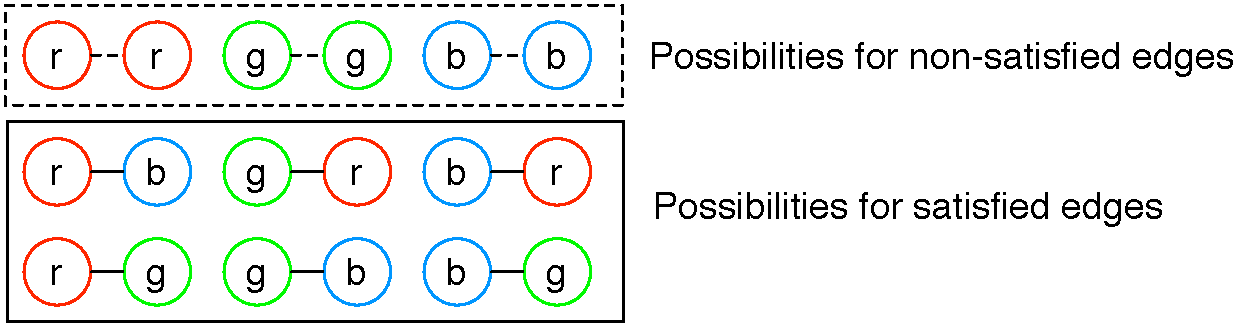
\includegraphics[width=\textwidth]{Figures/3_Color_Possibilities_Edges}
    \label{figure:3_Color_Possibilities_Edges}
\end{figure}


\[
	\text{Random Variable: } Z_{ij} =
    \left\{
    	\begin{array}{l l}
    		1 & \quad \text{if edge $e_{ij}$ is satisfied}\\

    		0 & \quad \text{otherwise}
    	\end{array}
    \right.
\]
\[
    \text{Number of satisfied edges}: Z = c^* · ∑_{(i,j)∈E(G)} Z_{ij}
\]
\[
    E[Z] =
    c^* · ∑_{(i,j)∈E(G)}E[Z_{ij}] =
    c^* · ∑_{(i,j)∈E(G)}Pr[e_{ij} \text{ is satisfied}] =
    \frac{6}{9} c^∗=
    \frac{2}{3} c^∗
\]

\section{Exercise 2 (3-Coloring Approximation Algorithm)}

Assume all edges are satisfiable, i.e. $c^∗ = |E|$. How can you turn your
algorithm into a $\frac{2}{3}$-approximation algorithm that is guaranteed to
find a solution satisfying at least $\frac{2}{3} c^∗$ edges? What is the
expected runtime of this extended algorithm?

\subsection{Solution}

We start by finding the probability $p$ that $≥ \frac{2}{3} c^∗$ edges are
satisfied.
\begin{align*}
    &p_{j}: \text{probability that exactly j edges are satisfied}; \quad
    p = ∑_{j≥2/3|E|}p_j\\
    & E[Z] =
    \frac{2}{3} |E| =
    ∑_{j<2/3|E|} j · p_j + ∑_{j≥2/3|E|} j · p_j ≤
    \frac{2|E|-1}{3} ∑_{j<2/3|E|} p_j + |E| ∑_{j≥2/3|E|} p_j =\\
    &= \frac{2|E|-1}{3} (1-p) + |E|·p ≤ \frac{2|E|-1}{3} + |E|·p\\
    &⇒ \frac{2}{3} |E| ≤ \frac{2|E|-1}{3} + |E|·p\\
    &\quad~~\frac{2}{3} |E| - \frac{2}{3} |E| + \frac{1}{3} ≤ |E|·p\\
    &\quad~~p≥\frac{1}{3·|E|}
\end{align*}

Since we find a solution satisfying $\frac{2}{3} c^∗$ edges, with a probability
$p≥\frac{1}{3·|E|}$, we use the algorithm from Section~\ref{section:Exercise1}
together with a routine which checks the number of satisfied edges (runtime:
$O(|E|)$, and run this code till we find an assignment which satisfies $≥
\frac{2}{3} c^∗$ edges. The expected run time of this algorithm is
$O(3·|E|)·O(|V|+|E|)=O(|E|^2+|E|·|V|)$.

\section{Exercise 6 (Cut Vertices)}

Let $G = (V, E)$ be a connected, undirected graph. A cut vertex of $G$ is a
vertex whose removal disconnects $G$. Describe a linear time, i.e., $O(|V | +
|E|)$, algorithm to identify all cut vertices of $G$.

\subsection{Solution}

The following algorithm is a slightly modified version of the pseudo-code
described in the document “Finding Cut Vertices and Biconnected Components with
Depth First Search”~\cite{Finding_Cut_Vertices}. More information about the
original algorithm by John Hopcroft and Robert Tarjan can be found at
Wikipedia~\cite{Wikipedia_Connected_Components}.

\paragraph{Pseudocode:}~

\begin{leftbar}
    \input{Code/cut_vertices}
\end{leftbar}

Figure~\ref{figure:Cut_Vertices}~\cite{Solutions_Exercise1_Hamboeck} shows the
result of the pseudo code applied to an example graph.

\begin{figure}[htbp]
    \caption{Example Graph with cut vertices C and D}
    \vskip 0.2cm
    \centering
    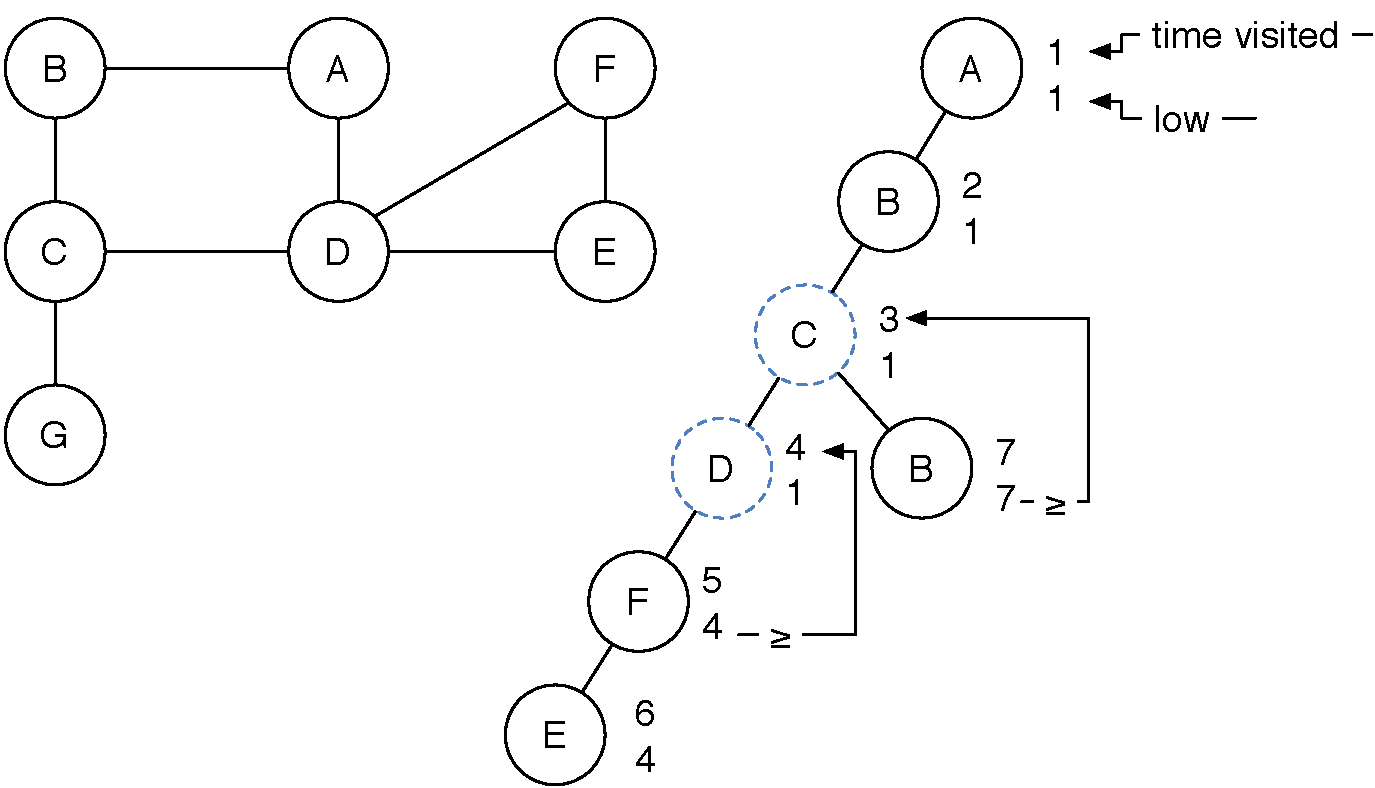
\includegraphics[width=0.9\textwidth]{Figures/Cut_Vertices}
    \label{figure:Cut_Vertices}
\end{figure}

\section{Exercise 7 (Planar Graphs)}

\begin{itemize}

    \item Show that $m ≤ 3n − 6$ holds for any simple planar graph with $n ≥ 3$
    vertices and $m$ edges.

    \item Show that $m ≤ 2n − 4$ holds for any simple planar bipartite graph
    with $n ≥ 3$ vertices and m edges.

    \item Use Euler’s formula to show that each simple, planar graph contains a
    vertex $v$ of degree $d(v) ≤ 5$.

\end{itemize}

\subsection{Solution}

\paragraph{Remark:} The solution for this exercise is basically a slightly
modified versions of the proofs from “Solution to exercises 1” by Thomas
Hamböck~\cite{Solutions_Exercise1_Hamboeck}.

\subsubsection{Exercise 7.1}

We need to show that $m ≤ 3n − 6$ holds for any simple planar graph with $n ≥
3$ vertices and $m$ edges.\\

We know that each edge in a simple planar graph is a border of two faces. We
also know that each face has to contain at least $3$ edges. From that knowledge
we conclude that the sum of the edges multiplied by $2$ is equal to the sum of
the edges of all faces counted together:
\begin{align*}
    2 · |E| = ∑_{i≥3} i · Fᵢ &\quad i…\text{Number of edges of the face }Fᵢ\\
                             &\quad F_i…\text{Number of Faces with i edges}
\end{align*}
From the fact that each face contains at least $3$ edges we conclude the
following:
\begin{align*}
      3 · ∑_{i≥3} Fᵢ    &≤ ∑_{i≥3} i · Fᵢ\\
      3 · |F|           &≤ 2 · |E| \quad \biggm| ~: 3\\
          |F|           &≤ \frac{2}{3} · |E|
\end{align*}

We now use Euler’s formula:
\[
    |V| - |E| + |F| = 2
\]

and insert the inequality from before:
\begin{align*}
    |V| - |E| + |F| = 2 &≤ |V| - |E| + \frac{2}{3} · |E| && \biggm| · 3\\
    6                   &≤ 3·|V| - |E|\\
    |E|                 &≤ 3·|V| - 6
\end{align*}

\subsubsection{Exercise 7.2}

To show that $m ≤ 2n − 4$ holds for any simple planar bipartite graph with $n ≥
3$ vertices and m edges we use basically the same arguments as in the example
before.\\

Instead of the minimum number of $3$ edges for each face, the number of
edges for a face in a bipartite graph is at least $4$ (a graph with a face
containing $3$ edges is never bipartite):
\begin{align*}
    2 · |E| = ∑_{i≥4} i · Fᵢ &\quad i…\text{Number of edges of the face }Fᵢ\\
                             &\quad F_i…\text{Number of Faces with i edges}
\end{align*}
The number of edges in each face is bigger or equal to $4$:
\begin{align*}
      4 · ∑_{i≥4} Fᵢ    &≤ ∑_{i≥4} i · Fᵢ\\
      4 · |F|           &≤ 2 · |E|\\
          |F|           &≤ \frac{1}{2} · |E|
\end{align*}
Insert the inequality into Euler’s formula:
\begin{align*}
      |V| - |E| + |F| = 2 &≤ |V| - |E| + \frac{1}{2} · |E| && \biggm| · 2\\
      4                   &≤ 2·|V| - |E|\\
      |E|                 &≤ 2·|V| - 4
\end{align*}

\subsubsection{Exercise 7.3}

We use Euler’s formula to show that each simple, planar graph contains a vertex
$v$ of degree $d(v) ≤ 5$.\\

We assume that all vertices have degree greater than $5$. This means the
average degree $d_{avg}$ has to be greater or equal to $6$:\\
\[
    d_{avg} = \frac{2|E|}{|V|} ≥ 6
\]
In the first sub-exercise we already used Euler’s formula to show that $E ≤
3·|V| - 6$ holds for each simple, planar graph with $|V|≥3$:
\begin{align*}
    |E|                 &≤ 3·|V| - 6    &&\biggm| ~· 2\\
    2·|E|               &≤ 6·|V| - 12   &&\biggm| ~: |V|\\
    \frac{2·|E|}{|V|}   &≤ 6 -\frac{12}{|V|} < 6\\
    d_{avg}             &< 6
\end{align*}
Since we showed that the average degree has to be smaller than $6$ we conclude
that a node with degree $5$ or smaller has to exist in the graph.

\section{Exercise 8 (Dijkstra’s Shortest Path Algorithm)}

Why is it not possible in general to apply Dijkstra’s shortest path algorithm
to get the longest path. Under which circumstances can the longest path be
computed efficiently?

\subsection{Solution}

Finding the longest path can be translated to finding the shortest path in a
copy of the graph, in which all edge weights are multiplied by $-1$. This might
lead to a graph which contains negative weight cycles. This in turn means that
the problem of finding the longest path is $\mathcal{NP}$
complete~\cite{Algorithmics_Slides} and can therefore not computed using an
polynomial time algorithm, like the Dijkstra algorithm.\\

Even in an acyclic graph the Dijkstra algorithm might not find the correct
maximum path. For example,
Figure~\ref{figure:Dijkstra_Counter_Example}~\cite{Dijkstra_Longest_Path} shows
an example where Dijkstra’s algorithm finds a path with weight $4$ ($A-B-C$)
from node $A$ to node $C$ instead of the correct path $A-D-C$ with length $6$.\\

\begin{figure}[htbp]
    \caption{
        An acyclic graph for which the Dijkstra algorithm does not find the
        correct maximum path
    }
    \vskip 0.2cm
    \centering
    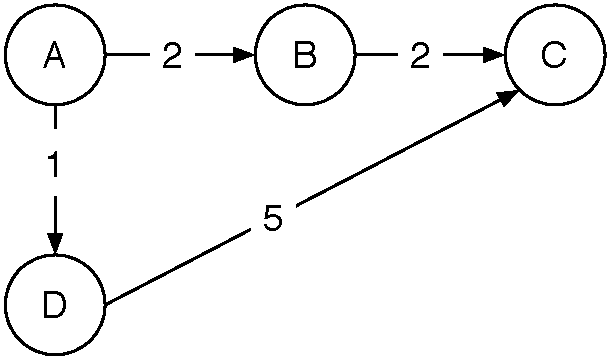
\includegraphics[width=0.4\textwidth]{Figures/Dijkstra_Counter_Example}
    \label{figure:Dijkstra_Counter_Example}
\end{figure}

The problem, lies within the „greedy” nature of the Dijkstra algorithm. If
we, for example, apply the Bellman-Ford algorithm on
Figure~\ref{figure:Dijkstra_Counter_Example}, using the maximum operator instead
of the minimum, we get the correct maximum path with length $6$ between the
nodes $A$ and $C$ (see Table~\ref{table:Bellman_Ford_Longest_Path}).\\

\begin{table}[htbp]
    \caption{
        Calculations for finding the longest path in
        Figure~\ref{figure:Dijkstra_Counter_Example} using the Bellman-Ford
        algorithm
    }
    \begin{center}
        \begin{tabular}{cccc}
            $δ_A$ & $δ_B$ & $δ_C$ & $δ_D$\\
            \hline
            0     &  ∞    &  ∞    &  ∞\\
            0     &  2    &  ∞    &  1\\
            0     &  2    &  4    &  6\\
            0     &  2    &  4    &  6\\
        \end{tabular}
    \end{center}
    \label{table:Bellman_Ford_Longest_Path}
\end{table}

In general the longest path can be computed in linear time if the graph is
acyclic~\cite{Wikipedia_Longest_Path}. However, the Dijkstra algorithm is in
general unable to find this longest path. Using the Bellman Ford
algorithm instead should work.

\section{Exercise 9 (Floyd-Warshal Algorithm)}

Apply the Floyd-Warshal algorithm as presented in the lecture to the given
graph.

\begin{center}
    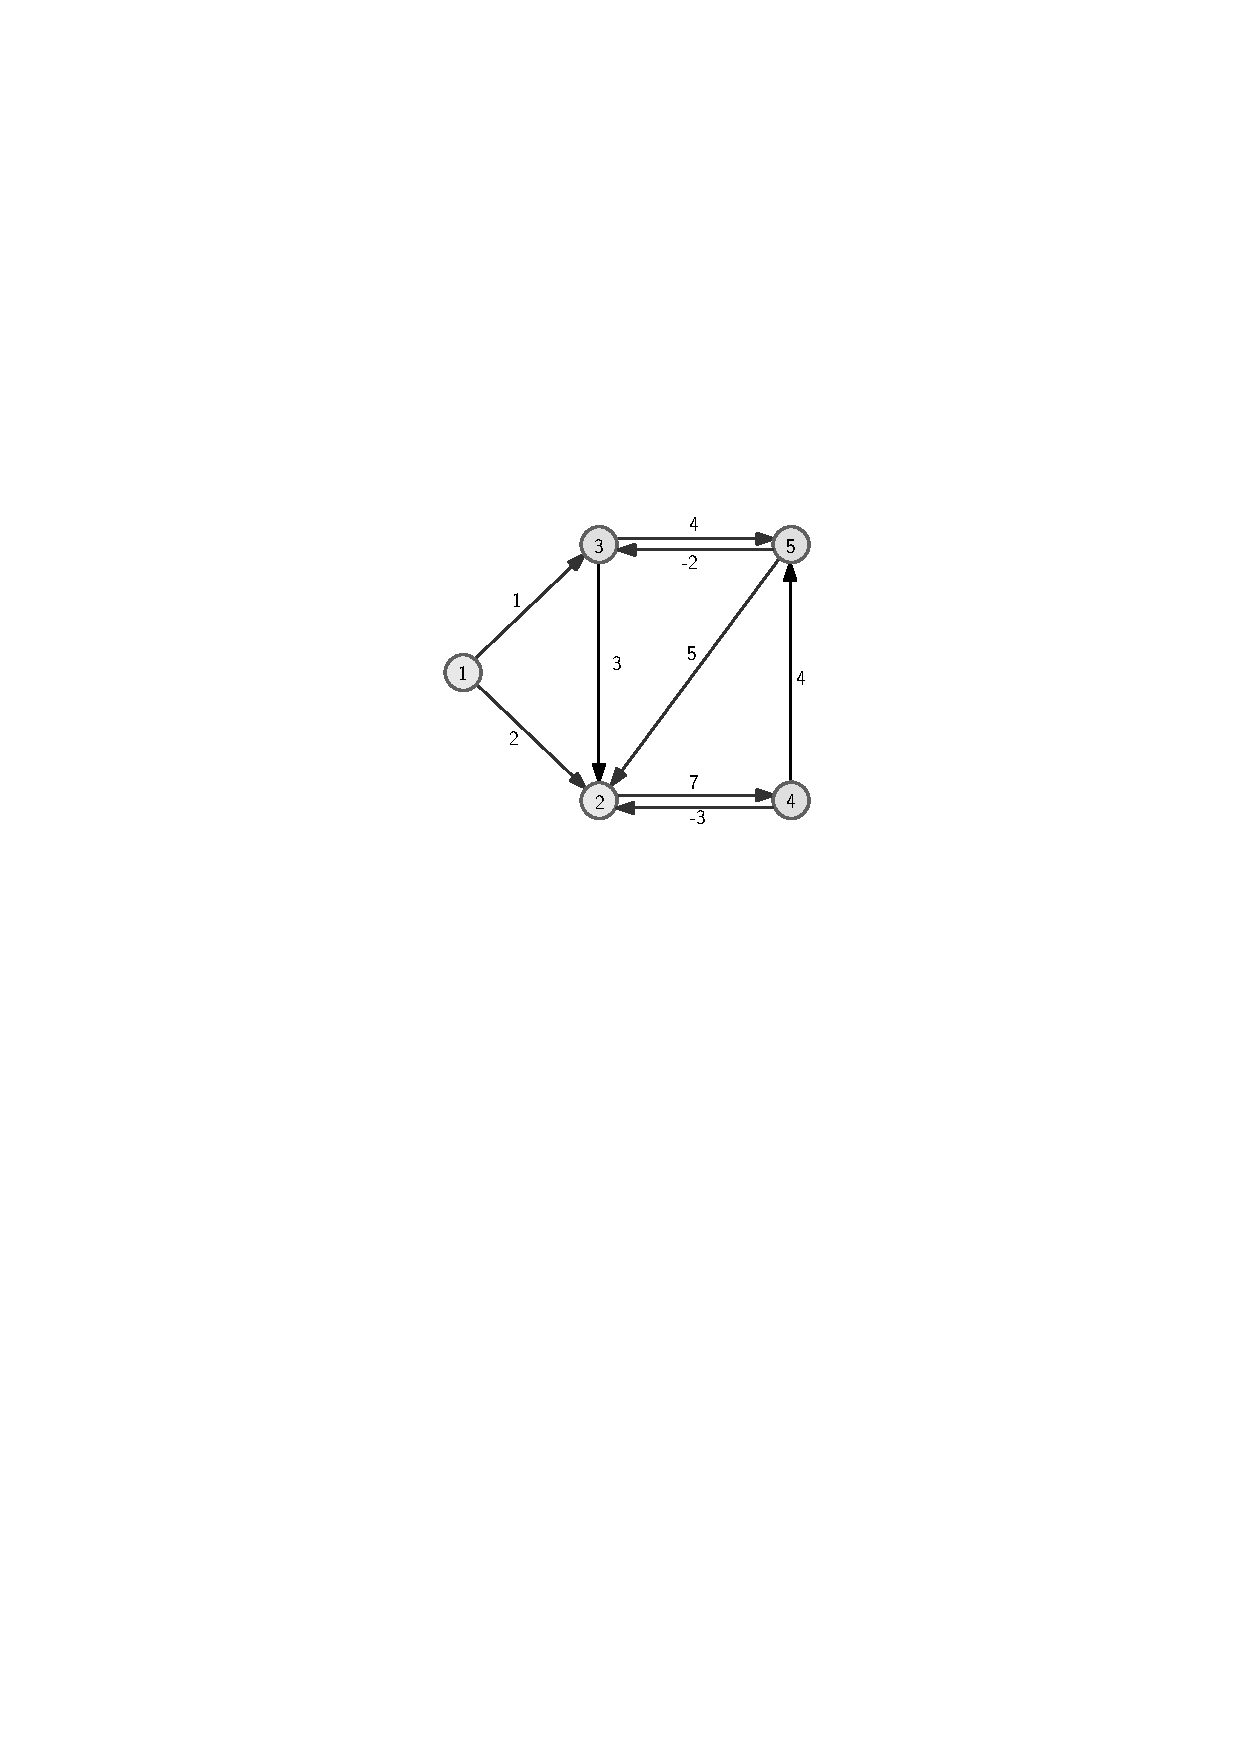
\includegraphics[width=0.5\textwidth]{Figures/Exercise_9}
\end{center}

\subsection{Solution}

\[
W = D^{(1)} =
\left(
    \begin{array}{ccccc}
        \highlight{0}   &
        \highlight{2}   &
        \highlight{1}   &
        \highlight{∞}   &
        \highlight{∞}   \\

        \highlight{∞}   &   0   &   ∞   &   7   &   ∞   \\
        \highlight{∞}   &   3   &   0   &   ∞   &   4   \\
        \highlight{∞}   &   -3  &   ∞   &   0   &   4   \\
        \highlight{∞}   &   5   &   -2  &   ∞   &   0   \\
    \end{array}
\right)
\]

\begin{minipage}[b]{0.5\linewidth}
\[
D^{(2)} =
\left(
    \begin{array}{ccccc}
        0   &   \highlight{2}   &   1   &   ∞   &   ∞   \\

        \highlight{∞}   &
        \highlight{0}   &
        \highlight{∞}   &
        \highlight{7}   &
        \highlight{∞}   \\

        ∞   &   \highlight{3}   &   0   &   ∞   &   4   \\
        ∞   &   \highlight{-3}  &   ∞   &   0   &   4   \\
        ∞   &   \highlight{5}   &   -2  &   ∞   &   0   \\
    \end{array}
\right)
\]
\end{minipage}
\begin{minipage}[b]{0.5\linewidth}
\[
D^{(3)} =
\left(
    \begin{array}{ccccc}
        0   &   2   &   \highlight{1}   &   9   &   ∞   \\
        ∞   &   0   &   \highlight{∞}   &   7   &   ∞   \\

        \highlight{∞}   &
        \highlight{3}   &
        \highlight{0}   &
        \highlight{10}  &
        \highlight{4}   \\

        ∞   &   -3  &   \highlight{∞}   &   0   &   4   \\
        ∞   &   5   &   \highlight{-2}  &   12   &   0  \\
    \end{array}
\right)
\]
\end{minipage}

\begin{minipage}[b]{0.5\linewidth}
\[
D^{(4)} =
\left(
    \begin{array}{ccccc}
        0   &   2   &   1   &   \highlight{9}   &   5   \\
        ∞   &   0   &   ∞   &   \highlight{7}   &   ∞   \\
        ∞   &   3   &   0   &   \highlight{10}  &   4   \\

        \highlight{∞}   &
        \highlight{-3}  &
        \highlight{∞}   &
        \highlight{0}   &
        \highlight{4}   \\

        ∞   &   1   &   -2  &   \highlight{8}   &   0   \\
    \end{array}
\right)
\]
\end{minipage}
\begin{minipage}[b]{0.5\linewidth}
\[
D^{(5)} =
\left(
    \begin{array}{ccccc}
        0   &   2   &   1   &   9   &   \highlight{5}   \\
        ∞   &   0   &   ∞   &   7   &   \highlight{11}  \\
        ∞   &   3   &   0   &   10  &   \highlight{4}   \\
        ∞   &   -3  &   ∞   &   0   &   \highlight{4}   \\

        \highlight{∞}   &
        \highlight{1}   &
        \highlight{-2}  &
        \highlight{8}   &
        \highlight{0}   \\
    \end{array}
\right)
\]
\end{minipage}

\begin{minipage}[b]{0.5\linewidth}
\[
D^{(6)} =
\left(
    \begin{array}{ccccc}
        0   &   2   &   1   &   9   &   5   \\
        ∞   &   0   &   9   &   7   &   11  \\
        ∞   &   3   &   0   &   10  &   4   \\
        ∞   &   -3  &   2   &   0   &   4   \\
        ∞   &   1   &   -2  &   8   &   0   \\
    \end{array}
\right)
\]
\end{minipage}
\begin{minipage}[b]{0.5\linewidth}
\end{minipage}

\section{Exercise 10 (Johnson’s Algorithm)}

Calculate the values $hᵢ$ and $\hat{w}_{ij}$ as it is done by Johnson’s
algorithm for the graph of exercise 9.

\subsection{Solution}

\begin{minipage}[b]{0.5\linewidth}
\[
A' =
\left(
    \begin{array}{cccccc}
        0   &   0   &   0   &   0   &   0   &  0    \\
        ∞   &   0   &   2   &   1   &   ∞   &  ∞    \\
        ∞   &   ∞   &   0   &   ∞   &   7   &  ∞    \\
        ∞   &   ∞   &   3   &   0   &   ∞   &  ∞    \\
        ∞   &   ∞   &   -3  &   ∞   &   0   &  4    \\
        ∞   &   ∞   &   5   &   -2  &   ∞   &  0    \\
    \end{array}
\right)
\]
\end{minipage}
\begin{minipage}[b]{0.5\linewidth}
\begin{center}
    \begin{tabular}{c|cccccc}
        &  $δ_s$ &  $δ₁$  &  $δ₂$  &  $δ₃$  &  $δ₄$  &  $δ₅$\\
    \hline
    0   &  0     &  ∞      &  ∞      &  ∞      &  ∞      &  ∞    \\
    1   &  0     &  0      &  0      &  0      &  0      &  0    \\
    2   &  0     &  0      &  -3     &  -2     &  0      &  0    \\
    3   &  0     &  0      &  -3     &  -2     &  0      &  0    \\
    4   &  0     &  0      &  -3     &  -2     &  0      &  0    \\
    5   &  0     &  0      &  -3     &  -2     &  0      &  0    \\
    \hline
        &  $h_s$ &  $h₁$  &  $h₂$  &  $h₃$  &  $h₄$  &  $h₅$\\
    \end{tabular}
\end{center}
\end{minipage}

\begin{figure}[htbp]
    \caption{Graph for Johnson's Algorithm with initial weights}
    \vskip 0.2cm
    \centering
    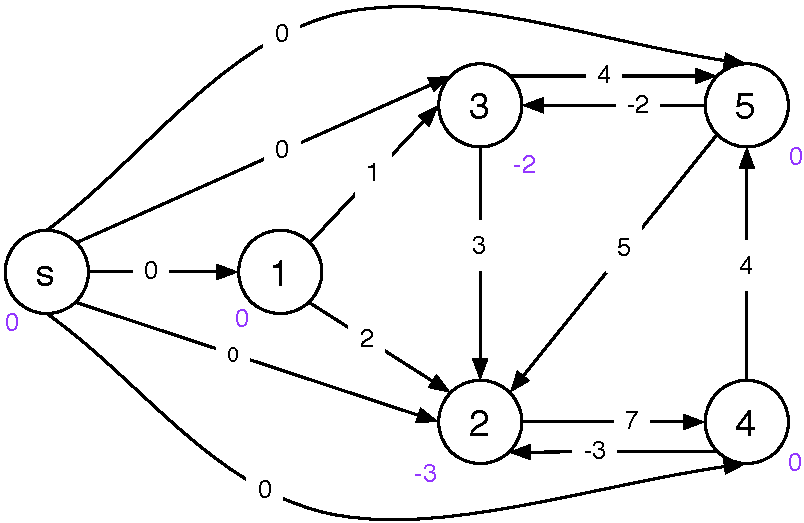
\includegraphics[width=0.8\textwidth]{Figures/Exercise_10_Initial}
    \label{figure:Exercise_10_Initial}
\end{figure}

\begin{figure}[htbp]
    \caption{
        Graph for Johnson's Algorithm with modified weight function
        $\hat{w}_{ij}$
    }
    \vskip 0.2cm
    \centering
    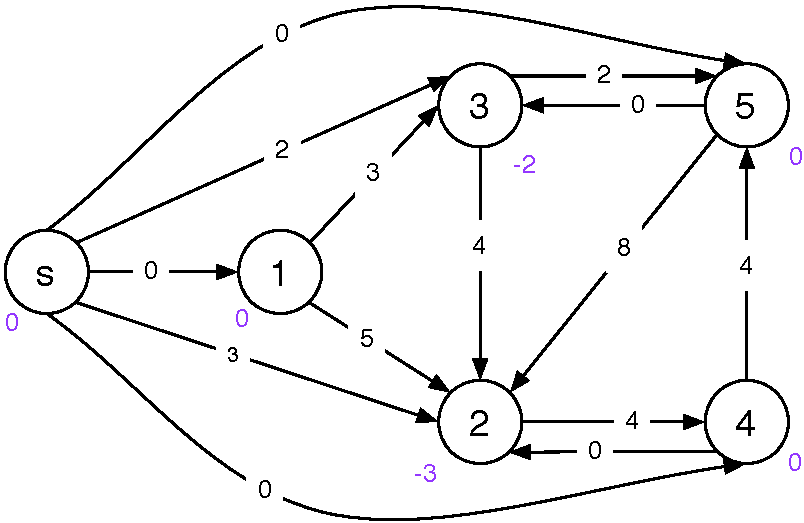
\includegraphics[width=0.8\textwidth]{Figures/Exercise_10_Modified_Weights}
    \label{figure:Exercise_10_Modified_Weights}
\end{figure}

\[
A =
\left(
    \begin{array}{cccccc}
       0   &   5   &   3   &   ∞   &  ∞    \\
       ∞   &   0   &   ∞   &   4   &  ∞    \\
       ∞   &   4   &   0   &   ∞   &  2    \\
       ∞   &   0   &   ∞   &   0   &  4    \\
       ∞   &   8   &   0   &   ∞   &  0    \\
    \end{array}
\right)
\]

\section{Exercise 11 (Modeling as Shortest Path Problem)}

The following table illustrates a number of possible duties for the drivers of
a bus company. We wish to ensure, at the lowest possible cost, that at least
one driver is on duty for each hour of the planning period (9 AM to 5 PM).
Formulate and solve this scheduling problem as shortest path problem.

\begin{center}
    \begin{tabular}{|c|c|c|c|c|c|c|c|c|}
        \hline
        Duty hours  & 9-13  & 9-11  & 12-15 & 12-17 & 14-17 & 13-16 & 16-17\\
        \hline
        Costs       & 30    & 18    & 21    & 38    & 20    & 22    & 9\\
        \hline
    \end{tabular}
\end{center}

\subsection{Solution}

We create a graph in which nodes represent the start and the end time of the
work hours of one bus driver. The edge between two nodes describes the cost of
the driver for the given hours.\\

Since it is alway possible that multiple bus drivers are on duty for a certain
amount of time we add edges with cost 0 between a certain hour and the hour
before. We now apply the Dijkstra algorithm on the resulting graph, shown in
Figure~\ref{figure:Bus_Driver_Schedule}.

\begin{figure}[htbp]
    \caption{Weighted graph for Exercise 11}
    \vskip 0.2cm
    \centering
    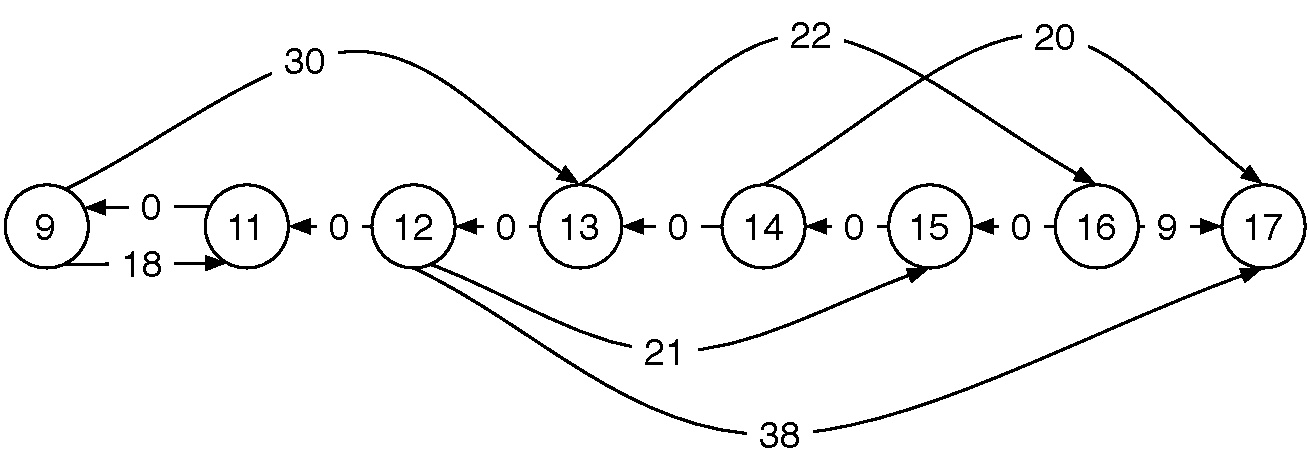
\includegraphics[width=\textwidth]{Figures/Bus_Driver_Schedule}
    \label{figure:Bus_Driver_Schedule}
\end{figure}

\begin{table}[htbp]
    % Highlight text with color
    \caption{Results of the Dijkstra algorithm, applied to
             Figure~\ref{figure:Bus_Driver_Schedule}}
    \begin{center}
        \begin{tabular}{cccccccc|cc}

            9 & 11 & 12 & 13 & 14 & 15 & 16 & 17 & Node & Previous\\
            \hline
            \highlight{0}
              & ∞  & ∞  & ∞  & ∞  & ∞  & ∞  & ∞  & 9    & — \\

              & \highlight{18}
                   & ∞  & 30 & ∞  & ∞  & ∞  & ∞  & 11   & 9 \\

              &    & ∞  & \highlight{30}
                             & ∞  & ∞  & ∞  & ∞  & 13   & 9 \\

              &    & \highlight{30}
                        &    & ∞  & ∞  & 52 & ∞  & 12   & 13 \\

              &    &    &    & ∞  & \highlight{51}
                                       & 52 & 68 & 15   & 12 \\

              &    &    &    & \highlight{51}
                                  &    & 52 & 68 & 14   & 15 \\

              &    &    &    &    &    & \highlight{52}
                                            & 68 & 16   & 13 \\

              &    &    &    &    &    &    & \highlight{61}
                                                 & 17   & 16 \\
        \end{tabular}
    \end{center}
    \label{table:Label}
\end{table}

The shortest path and therefore the schedule with the minimum cost of „61” is:

\begin{center}
    \begin{tabular}{c|ccc}
        hours & 9-13 & 13-16 & 16-17\\
        costs & 30     & 22  & 9\\
    \end{tabular}
\end{center}

\section{Exercise 12 (Delay Constrained Shortest Path)}

Suppose we are given a network $N=(G,w,d), G=(V,A)$, where $w:A→ℤ^+$ and
$d:A→ℤ^+$. The values $w_{ij}$ correspond to arc weights, $d_{ij}$ correspond
to delays, i.e., using the arc $(i,j)$ requires $d_{ij}$ time. We are further
given a positive number $D ∈ ℕ$, the delay constraint. Develop an
efficient, i.e., $O(D · |A|)$, algorithm to find a shortest path $P$ from some
arbitrary source node $s$ to some arbitrary target node $t$ which does not
exceed the global delay constraint $D$, i.e., $∑_{(i,j) ∈ P} d_{ij} ≤ D$.

\subsection{Solution}

To solve the constrained shortest path problem we use a modified version of the
Bellman-Ford Algorithm. Instead of iterating over the edges we iterate over the
delay. This means that we get the shortest path with a delay shorter or equal
to $i$ in round $i$.\\

To get the shortest path to some node $v$ we check all incoming edges to a
node. Let us assume the delay of the incoming arc $(u,v)$ is $d_{uv}$. We check
now if the weight of the shortest path to node $u$ in round $i-d_{uv}$ plus the
weight of the arc is smaller than the current shortest path $u$. If this is the
case we replace the shortest path to node $u$ with the new value.\\

We now apply this algorithm to the graph shown in
Figure~\ref{figure:Delay_Shortest_Path}. We use node “A” as source which leads us to the values given in Table~\ref{figure:Delay_Shortest_Path}.\\

\begin{table}[htbp]
    \caption{
        Shortest Delay Constrained Paths
        forFigure~\ref{figure:Delay_Shortest_Path}
    }
    \begin{center}
        \begin{tabular}{c|cccccc}
            Delay  &  $δ_A$ &  $δ_B$  &  $δ_C$  &  $δ_D$  &  $δ_E$  &  $δ_F$\\
            \hline
            0      &  0     &  ∞      &  ∞      &  ∞      &  ∞      &  ∞\\
            1      &  0     &  ∞      &  ∞      &  ∞      &  ∞      &  ∞\\
            2      &  0     &  ∞      &  1      &  ∞      &  ∞      &  ∞\\
            3      &  0     &  1      &  1      &  ∞      &  ∞      &  ∞\\
            4      &  0     &  1      &  1      &  ∞      &  3      &  ∞\\
            5      &  0     &  1      &  1      &  ∞      &  3      &  ∞\\
            6      &  0     &  1      &  1      &  11     &  3      &  ∞\\
            7      &  0     &  1      &  1      &  4      &  3      &  ∞\\
            8      &  0     &  1      &  1      &  4      &  3      &  12\\
            9      &  0     &  1      &  1      &  4      &  3      &  5\\
            …      &  …     &  …      &  …      &  …      &  …      &  …\\
            13     &  0     &  1      &  1      &  4      &  3      &  5\\
            14     &  0     &  1      &  1      &  4      &  3      &  4\\
        \end{tabular}
    \end{center}
    \label{table:Delay_Shortest_Path}
\end{table}

To get the shortest path to a certain node we just select $δ$ for this node and
calculate the way back.\\

For example, lets us assume we want to get the shortest path to node $F$ with
the delay constraint $9$. We see that the value for the shortest path ($5$) in
column $δ_F$ just changed from the value in the row before. This means we that
in the step before we selected a new edge. This edge has to be $(D,F)$ with
weight $1$, since the delay of the other possible edge $(E,F)$ is larger than
the delay constraint $9$.\\

We now go to the column for the shortest path to $D$ and check in which row the
value changed from $4$ to a higher value. This was the case in the row with
delay $7$. This in turn means that we selected edge $(B,D)$ in the step
before.\\

We now check the column for $B$ and after that the column for $C$. In the end
we get the shortest path $A-C-B-D-F$ to the node $F$, if the we restrict the
delay constraint to a maximum value of $9$.

\begin{figure}[htbp]
    \caption{Example graph for the Delay Constrained Shortest Path problem}
    \vskip 0.2cm
    \centering
    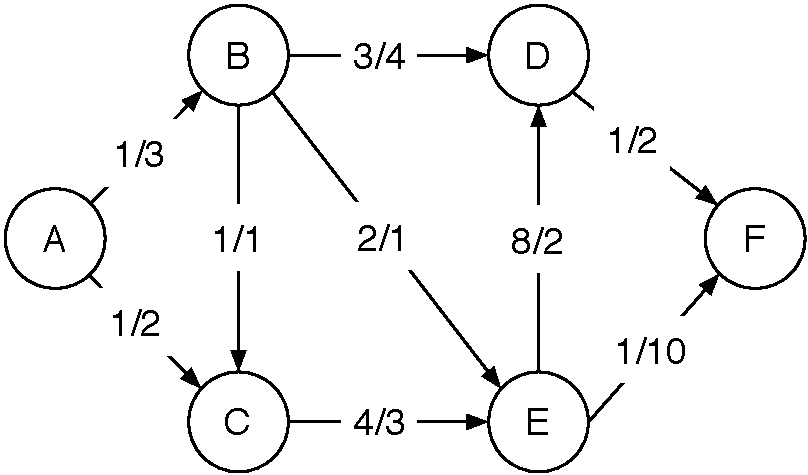
\includegraphics[width=0.7\textwidth]{Figures/Delay_Shortest_Path}
    \label{figure:Delay_Shortest_Path}
\end{figure}

\chapter{Exercise Session 2}

\section{Exercise 1 (Max-Flow Min-Cut Theorem)}

Let $f$ be a feasible flow in the flow network $N = (V,A,ς,s,t)$. Show for all
sets of nodes $S ⊂ V$ with $s,t ∉ S$ that:

\[
    f(S, \bar{S}) − f(\bar{S}, S) = 0 \quad (\bar{S} = V ~\backslash~ S).
\]

\subsection{Solution}

\begin{align*}
    \text{Flow conservation: } &
    ∑_{v ∈ V} f(u,v) = 0 \quad ∀ u ∈ V ~\backslash~ \{s, t\}\\
    f(S,V) &=
        ∑_{u ∈ S} \underbrace{∑_{v ∈ V} f(u, v)}_{=0} = ∑_{u ∈ S} 0 = 0 \\
    f(S, V) &=
        \underbrace{f(S,S)}_{=0} + f(S, \bar{S}) = 0 ⇒ f(S,\bar{S}) = 0 \\[5pt]
    \text{Skew Symmetry: }& f(u,v) = - f(v,u) \quad ∀ u,v ∈ V\\[2pt]
    f(S, \bar{S}) &= - f(\bar{S}, S) = 0 \\
    f(S, \bar{S}) − f(\bar{S}, S) &= 0   \\
    0 - 0 &= 0
\end{align*}

\section{Exercise 3 (Maximum Flow with Lower Bounds)}

Find in the given flow network $N$ with lower bounds.

\begin{enumerate}[a)]
    \item a feasible flow $f$
    \item a maximum flow $f^+$ in the residual graph $G_f$ based on $f$
    \item combine $f$ and $f^+$ to a maximum flow $f^∗$ for $N$.
\end{enumerate}

\begin{center}
    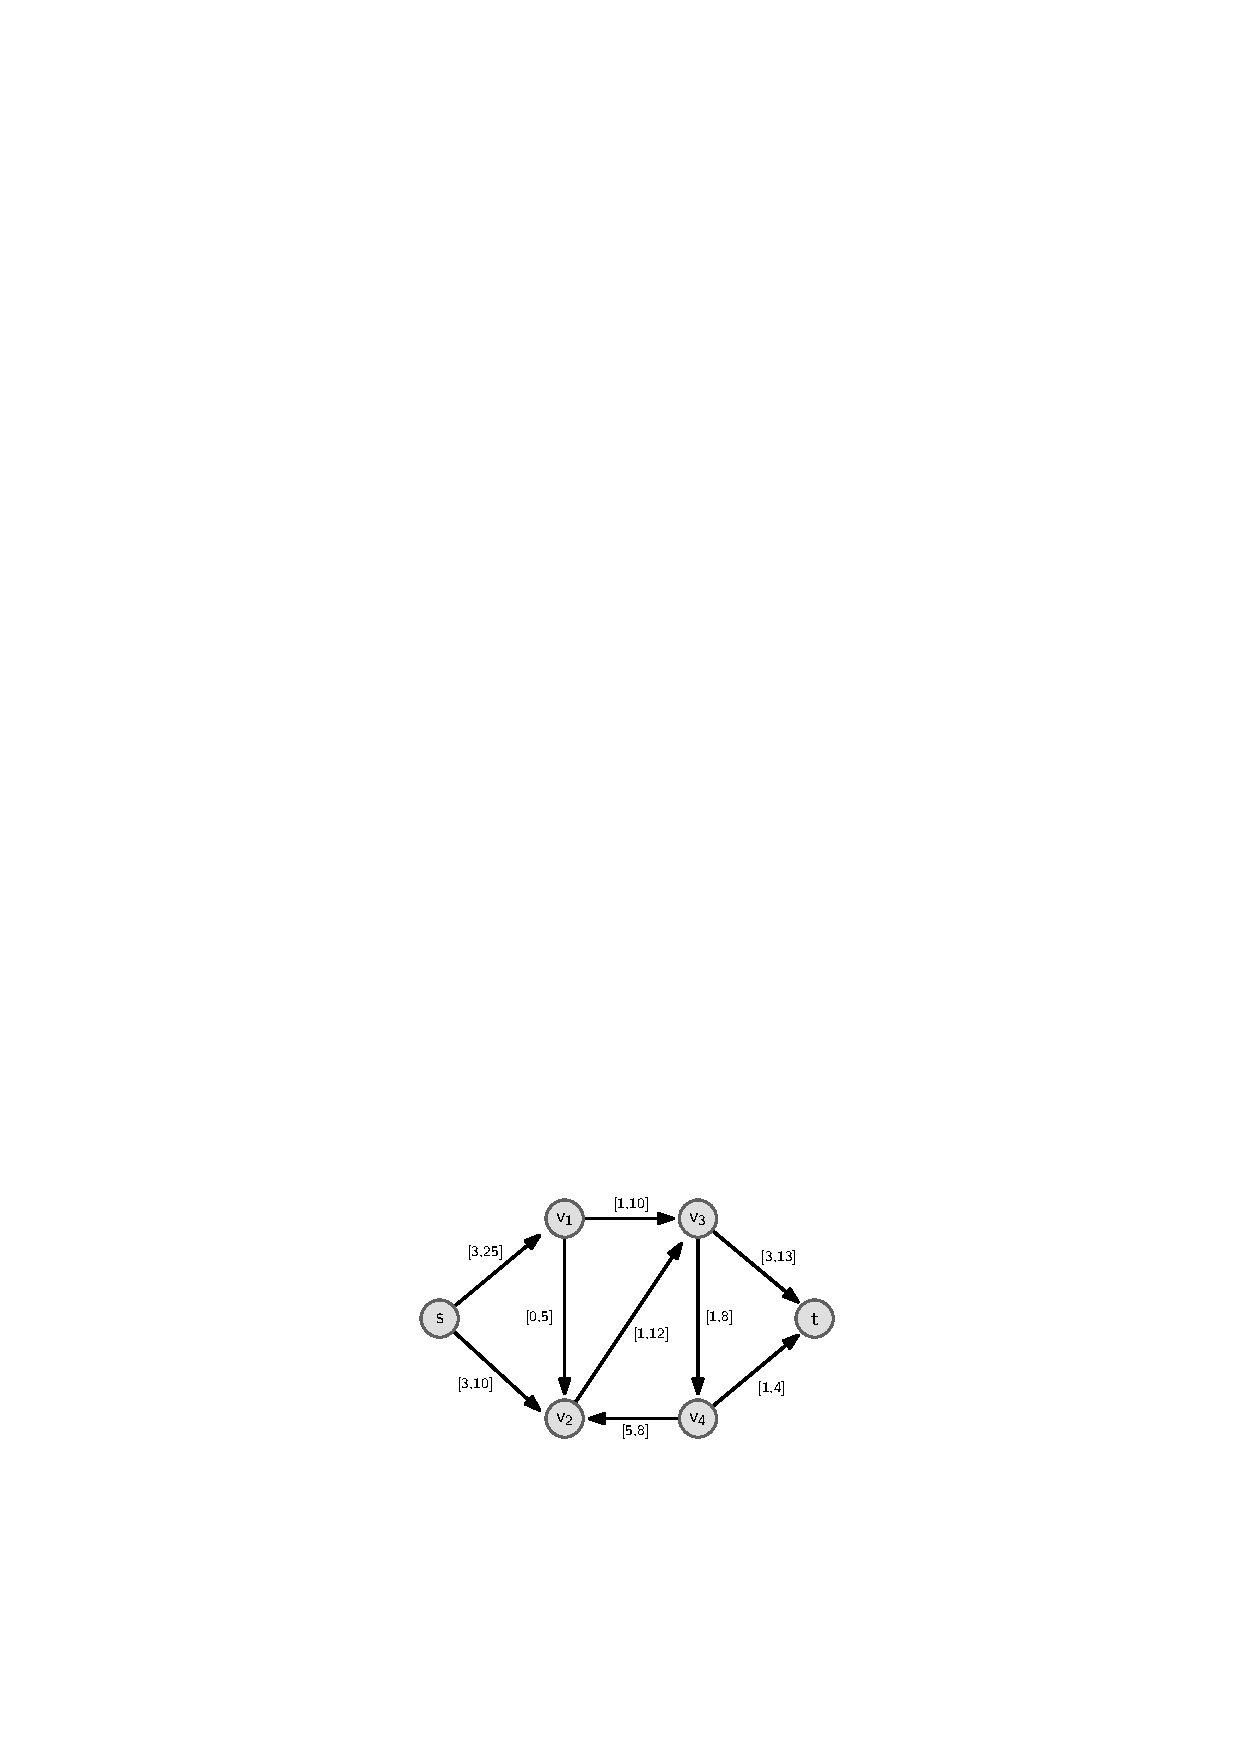
\includegraphics[width=0.5\textwidth]{Figures/Exercise_2_3}
\end{center}

\subsection{Solution}

\paragraph{a) Feasible Flow}

\begin{center}
    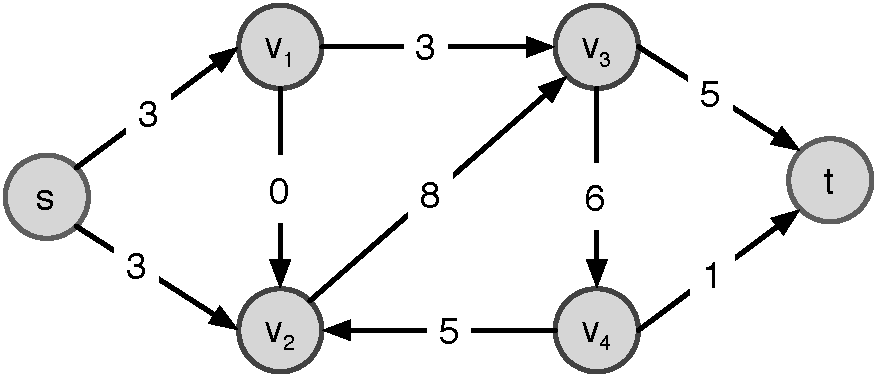
\includegraphics[width=0.5\textwidth]{Figures/Exercise_2_3_a}
\end{center}

\paragraph{b) Residual Graph $G_f$ with flow $f^+$}

\begin{center}
    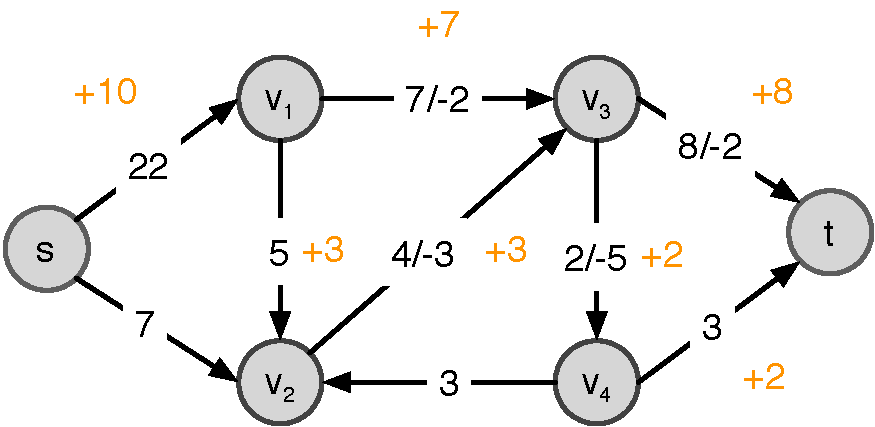
\includegraphics[width=0.5\textwidth]{Figures/Exercise_2_3_b}
\end{center}

\paragraph{c) Maximum Flow}

\begin{center}
    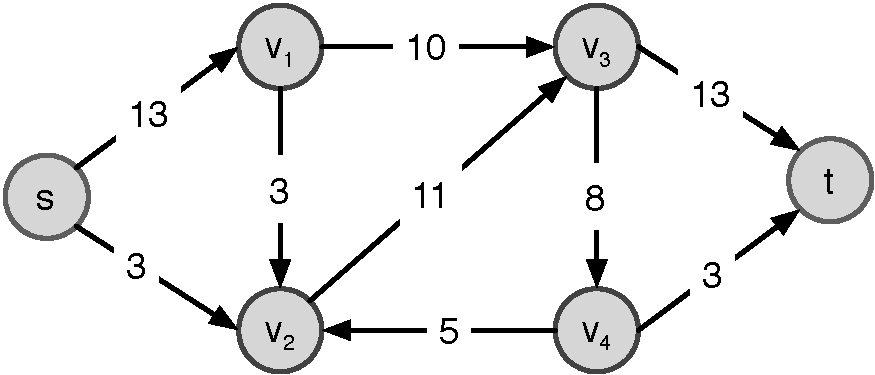
\includegraphics[width=0.5\textwidth]{Figures/Exercise_2_3_c}
\end{center}

\section{Exercise 4 (Maximum Flow with Lower Bounds)}

Given is a flow network $N$ with nonnegative lower capacity bounds. Find an
algorithm for combining a feasible flow f with a maximum flow $f^+$ in $G_f$ to
a maximum flow $f^∗$ in the original network $N$. Consider that there can be
both arcs $(u, v)$ and $(v, u)$ with different lower and upper capacity bounds.
(cf. Ex. 3).

\subsection{Solution}

We can just combine the maximum flow $f^*$ and the feasible flow $f^+$ by
adding them. Since there exists the possibility that the maximum flow for a
certain edge is exceeded we use the following algorithm to fix the combination
of the flows~\cite{Informatik_Forum_Combine_Flows}:

\begin{leftbar}
    \input{Code/combine_flows}
\end{leftbar}

We now show that this algorithm does not change the flow of an edge $b=(u,v)$,
in such a way that the flow of this node is smaller than the minimum capacity
of the edge. Let us say that $a=(v,u)$ is the edge where the flow was to large
and therefore had to be reduced.
\begin{align*}
    f'(x) &= f(x) + f^+(x)\\[10pt]
    \text{Assumption: } &∃ f'(b) - x < ς^L(b)\\[10pt]
    x &> f'(b) - ς^L(b)\\
    x &= f'(a) - ς^U(a)\\
    f'(a) - ς^U(a) &> f'(b) - ς^L(b)\\
    0 &> (ς^U(a) - f'(a)) + f'(b) - ς^L(b)\\
    0 &> r_{f'}(a)
\end{align*}

\section{Exercise 7 (A* Algorithm)}

Perform the $A∗$ algorithm on the following graph in order to find a shortest
path from $s$ to $t$. In which order are the nodes expanded, and when are which
nodes reached? Show the content of the priority queue at each iteration.

\begin{center}
    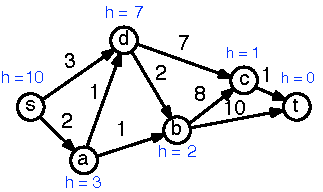
\includegraphics[width=0.6\textwidth]{Figures/Exercise_2_7}
\end{center}

\subsection{Solution}

\begin{table}[htbp]
    \caption{$A*$ algorithm applied to the graph of Exercise 7}
    \begin{center}
        \begin{tabular}{lll}
            Step & Calculations for $f'$    & Priority Queue\\
            \hline
            1    &                          & \highlight{(s, 10)}\\
            2    & (a, 2+3), (d, 3+7)       & \highlight{(a, 5)}, (d, 10)\\
            3    & (b, 3+2), (d, 3+7)       & \highlight{(b, 5)}, (d, 10)\\
            4    & (c, 11+1), (t, 13+0)     & (c, 12), \highlight{(d, 10)},
                                              (t, 13)\\
            5    & (b, 5+2), (c, 10+1)      & \highlight{(b, 7)}, (c, 11),
                                              (t, 13)\\
            6    & (c, 13+1), (t, 15)       & \highlight{(c, 11)}, (t, 13)\\
            7    & (t, 11+0)                & \highlight{(t, 11)}\\
        \end{tabular}
    \end{center}
    \label{table:A_Star}
\end{table}

\section{Exercise 8 (A* Algorithm for 8-Puzzle)}

Consider the 8-Puzzle discussed in the lecture. Show whether or not the two
suggested heuristics $h₁$ and $h₂$ are admissible and/or monotonic.

\subsection{Solution}

\paragraph{Heuristic 1: Number of Tiles in wrong position}

\subparagraph{Admissible}

Yes, since we need at least number of tiles in wrong position moves to get a
solution. The heuristic is optimistic (lower bound).

\subparagraph{Monotonic}

No, since we might need to move a tile to get to our solution which will
increase the heuristic value (see
Figure~\ref{figure:Exercise_2_8_h1_Monotonicity}).

\begin{figure}[htbp]
    \caption{$h₁$ is not monotonic}
    \vskip 0.2cm
    \centering
    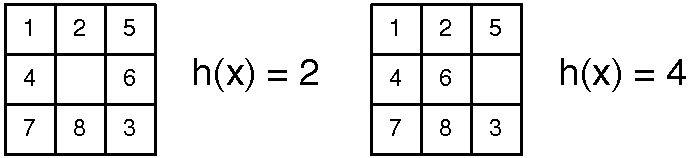
\includegraphics[width=0.5\textwidth]{Figures/Exercise_2_8_h1_Monotonicity}
    \label{figure:Exercise_2_8_h1_Monotonicity}
\end{figure}

\paragraph{Heuristic 2: Sum of the Manhatten distance of each tile to its
target location}

\subparagraph{Admissible}

Yes, since we need to move each tile at least “Manhatten distance” times.

\subparagraph{Monotonic}

No since we might need to move a tile to get to the solution, which will
increase the heuristic value (see
Figure~\ref{figure:Exercise_2_8_h2_Monotonicity}).

\begin{figure}[htbp]
    \caption{$h₁$ is not monotonic}
    \vskip 0.2cm
    \centering
    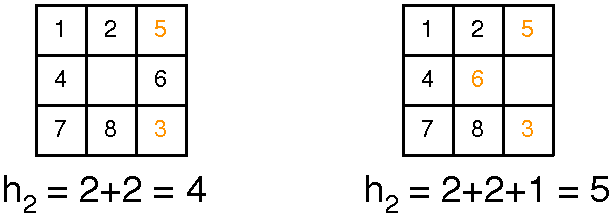
\includegraphics[width=0.5\textwidth]{Figures/Exercise_2_8_h2_Monotonicity}
    \label{figure:Exercise_2_8_h2_Monotonicity}
\end{figure}

\section{Exercise 9 (A* Algorithm for an Euclidean Graph)}

Consider an undirected graph whose nodes correspond to points in the Euclidean
plane. Instead of applying the Euclidean distance in a heuristic $h(x)$, we use
its square, i.e. $h(x) = (x₁ − t₁)² + (x₂ − t₂)²$, where $x = (x₁, x₂) ∈ V$ is
an arbitrary node and $t = (t₁, t₂)$ the target node. What might be a
motivation for doing this? Is the corresponding $A∗$ algorithm still guaranteed
to yield a shortest path? Prove or disprove this. How about monotonicity?

\subsection{Solution}

The squared Euclidean distance might be used to progressively place greater
weight on points that are farther apart. This means that $A∗$ should check out
less nodes and therefore finish faster~\cite{Wikipedia_Euclidean_Distance}.
Another reason for using the square euclidean distance might be the relative
large computational cost of taking the square root of a
number~\cite{Amit_A_Star}.\\

Figure~\ref{figure:Exercise_2_9_Monotonicity} shows that the heuristic is not
monotonic.

\begin{figure}[htbp]
    \caption{This graph shows that the square euclidean distance is not a
             monotonic heuristic}
    \vskip 0.2cm
    \centering
    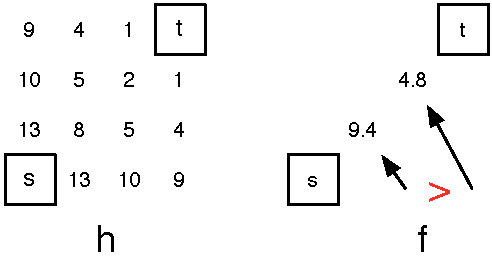
\includegraphics[width=0.5\textwidth]{Figures/Exercise_2_9_Monotonicity}
    \label{figure:Exercise_2_9_Monotonicity}
\end{figure}

The heuristic is not admissible since it returns an \emph{upper bound} for the
distance to a certain node. If we use the squared euclidean distance as
heuristic in the $A∗$ algorithm we might not always get the shortest path as
Figure~\ref{figure:Exercise_2_9_Wrong_Path} shows.\\

\begin{figure}[htbp]
    \caption{Using the squared euclidean distance as heuristic might lead to a
             wrong result for the shortest path}
    \vskip 0.2cm
    \centering
    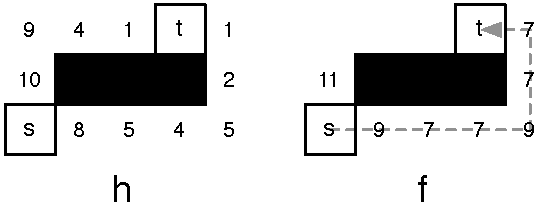
\includegraphics[width=0.5\textwidth]{Figures/Exercise_2_9_Wrong_Path}
    \label{figure:Exercise_2_9_Wrong_Path}
\end{figure}


\section{Exercise 10 (Cardinality Bipartite Matching)}
\label{section:Exercise_2_10}

Apply the algorithm for finding a maximum cardinality matching to the following
bipartite graph and explain each step.

\begin{center}
    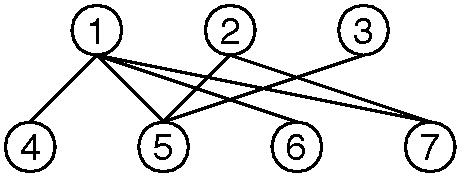
\includegraphics[width=0.5\textwidth]{Figures/Exercise_2_10}
\end{center}

\subsection{Solution}

Figure~\ref{figure:Exercise_2_10_Maximum_Matching} the steps taken to find the
maximum bipartite matching in the given graph. Since there are usually multiple
paths from U' to W' there are also multiple possibilities to find the maximum
matching.

\begin{figure}[htbp]
    \caption{Application of the “Cardinality Bipartite Matching” algorithm}
    \vskip 0.2cm
    \centering
    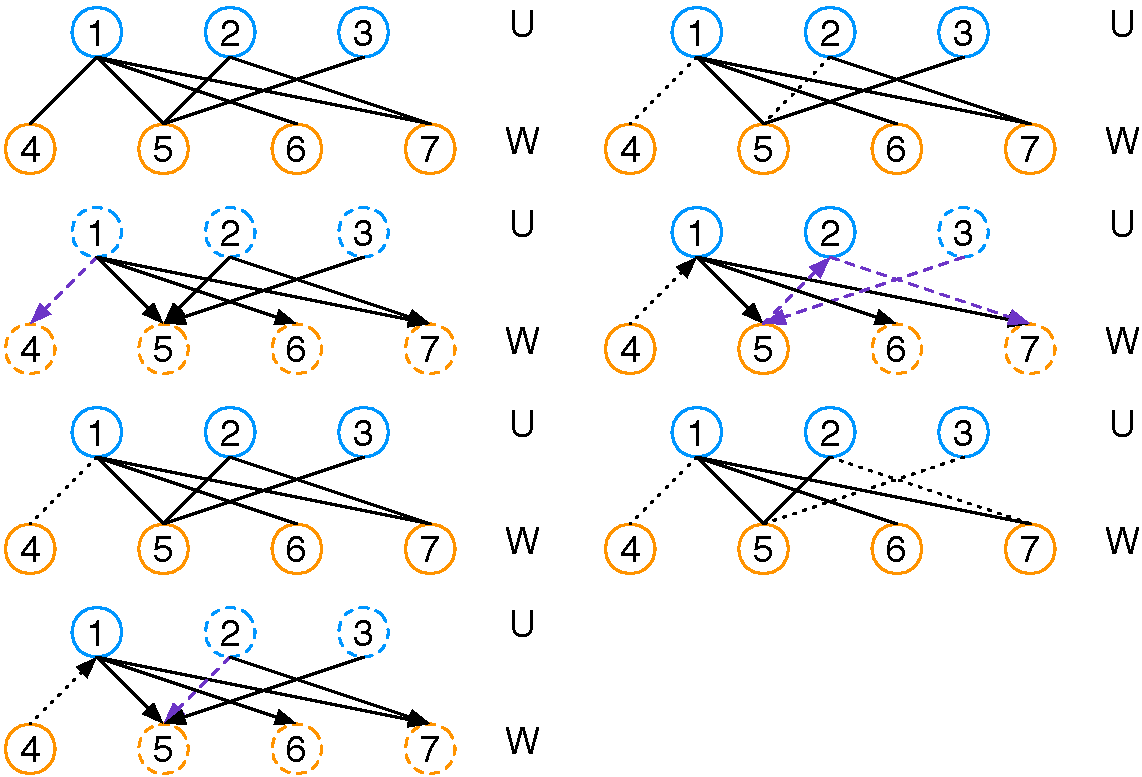
\includegraphics[width=\textwidth]{Figures/Exercise_2_10_Maximum_Matching}
    \label{figure:Exercise_2_10_Maximum_Matching}
\end{figure}

\section{Exercise 11 (Cardinality Bipartite Matching / Vertex Cover)}

Show that a minimum vertex cover can be found in a bipartite graph in
polynomial time.

\subsection{Solution}

We already know that we can find a maximum matching for a bipartite graph in
polynomial time. We now need to show that we can use this maximum matching to
get a minimum vertex cover.\\

For this purpose we partition the nodes of the graph into sets
$Sᵢ$~\cite{Wikipedia_Koenigs_Theorem}. The set $S₀$ contains all nodes which
are not part of the matching. After that we add all nodes which are adjacent to
the nodes $S₀$ to the set $S₁$. The edges between the set $S₀$ and $S₁$ are
obviously not contained in the matching. For the set $S₂$ we take all nodes
adjacent to the nodes contained in $S₁$ which are part of the matching. For
$S_3$ we take all nodes which were not already selected and are not part of the
matching. We continue this approach till all nodes are part of one set $Sᵢ$.\\

We get the minimal vertex cover by using all nodes contained in the odd sets.
Since one endpoint of a matched edge is contained in an even numbered set and
the other one in an odd numbered set, the cardinality of of the matching is
equal to the cardinality of our minimum vertex cover. König’s Theorem states
that this is indeed the correct cardinality for the minimum vertex cover.\\

Figure~\ref{figure:Exercise_2_11} shows the partitioning of a bipartite graph
using the described algorithm.

\begin{figure}[htbp]
    \caption{Minimal Vertex Cover for the graph from
             Exercise~\ref{section:Exercise_2_10}}
    \vskip 0.2cm
    \centering
    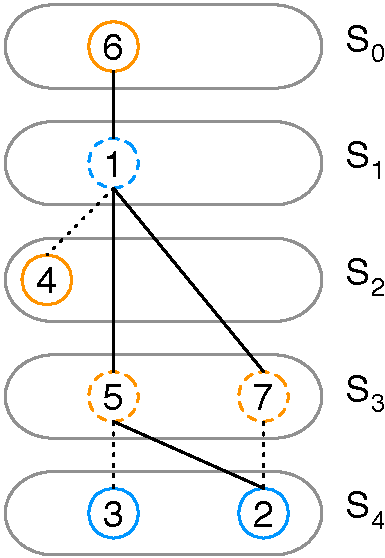
\includegraphics[width=0.3\textwidth]{Figures/Exercise_2_11}
    \label{figure:Exercise_2_11}
\end{figure}

We now have to show that the chosen vertices indeed are a correct vertex cover.
Since we have taken exactly one endpoint of each matched node we know that all
matched edges are covered. All unmatched edges are also covered if there are no
unmatched edges between node in an even numbered set. This can not be the case
since otherwise we could use this edge to get a larger matching. If there would
be a edge connecting two vertices $u$ and $v$ in an even numbered subset it
would join two alternating paths and we could get a larger matching by
switching the edges of this new path.

% -- Bibliography --------------------------------------------------------------

% Set section format for bibliography
\titleformat{\chapter}{\sffamily\bfseries}{}{0pt}{}[{\color{aqua}\hrule}]
% Display bibliography
\printbibliography

\end{document}
